\documentclass[a4paper]{article}
\usepackage{geometry}
\geometry{a4paper, scale=0.9}
\usepackage{lipsum} %This package just generates Lorem Ipsum filler text. 
\usepackage{fullpage} % changes the margin
\usepackage{mathpazo}
\usepackage{multicol}
\usepackage{enumerate, eucal}
\usepackage{listings}
\usepackage{xcolor}
\usepackage{amsmath,amsfonts,amsthm, amssymb} % Math packages
\usepackage{graphicx}
\usepackage{extarrows}
\usepackage{attachfile}

\begin{document}
%Header-Make sure you update this information!!!!
\noindent
\large \textbf{Homework 1} \hfill \textbf{Xun Gong(517020910141} \\
\normalsize {\bf CS 259 @ SJTU} \hfill ACM Class, Zhiyuan College, SJTU\\
Prof.~{\bf David Bindel} \hfill Due Date: May 29, 2019\\
TA.~{\bf Zhou Fan} \hfill Submit Date: \today

\section*{Problem 1: Regularized residual}

\subsection*{(1)}

\begin{align*}
&\mathcal{L} = ||Ax - b||^2 + \lambda ||x||^2 + \mu (b - Ax - r) \\
&\delta \mathcal{L} = \delta ||Ax - b||^2 + \lambda * \delta ||x||^2 
                    + \delta \mu A^T (b - Ax - r) - \mu A \delta x \\
&\delta \mathcal{L} = 2*\delta x^T (A^T A x - A^T b - \lambda x - \mu A^T) 
                    + delta \mu (b - Ax - r) = 0\\
\end{align*}

$$\begin{cases}
    b - Ax - r = 0\\
    A^T (Ax - b) - \lambda x = 0 \\
\end{cases}$$

\subsection*{(2)}

\begin{align*}
& b - Ax - r = 0\\
& A^T r - \lambda x = 0 \\
&\therefore r = (\frac{1}{\lambda}A A^T + 1)^{-1} b \\
\end{align*}

\subsection*{(3)}

\begin{align*}
& \frac{1}{\lambda}A A^T + 1 = \frac{b}{r} \\
& \text{diff equation: } -\frac{1}{\lambda^2} A A^T d\lambda = - \frac{b}{r^2} \\
& \frac{dr}{d\lambda} = \frac{A A^T * r^2}{b * \lambda^2} \\
& \text{From (2): } \frac{dr}{d\lambda} = \frac{A A^T * b}{\lambda^2} 
                    (\frac{1}{\lambda} A A^T + 1)^2\\
\end{align*}


\section*{Problem 2: Modified Landweber}

\subsection*{(1)}

\begin{align*}
    & x^{k+1} = G(x^k) = x^k - \frac{\alpha}{k+1}A^T(Ax^k-b) \\
    & e^{k+1} = G(x^* + e^k) - G(x^*) \\
    & \therefore e^{k+1} = x^* + e^k - \frac{\alpha}{k+1}A^T(Ax^* + Ae^k - b) - x^* \\
    & \therefore e^{k+1} = (1 - \frac{A^T A}{k+1} \alpha) e^k \\
    & \text{Let Constant } C = A^T A \alpha > 0 \\
    & \therefore e^{k+1} = (1 - \frac{C}{k+1}) e^k < (1 - \frac{C}{k+1})^{k+1} e^0 \\
    & \therefore e^k \text{ is decreasing.} \\
\end{align*}

\subsection*{(2)}

\begin{align*}
    & \text{Let } x^0 = 0 \\
    & x^1 = \alpha A^T b = a_1 \alpha A^T b ,\ &a_1 = I \\
    & x^2 = x^1 - \frac{1}{2} (\alpha A^T A x^1 - \alpha A^T b ) \\ 
    & x^2 = x^1 + \frac{1}{2} ( - \alpha A^T A a_1 \alpha A^T b + \alpha A^T b ) \\
    & x^2 = x^1 + \frac{1}{2} (I - \alpha A^T A a_1 ) \alpha A^T b
            = a_1 \alpha A^T b  + a_2 \alpha A^T b,\ &a_2 = \frac{1}{2} (I - \alpha A^T A) \\
    & x^3 = (a_1 + a_2 + a_3) \alpha A^T b, a_3 = \frac{1}{3} (I - \alpha A^T A) (I - \frac{1}{2} \alpha A^T A)\\
    & \quad 3*a_3 = I - \alpha A^T A (a_1 + a_2) \\
    & \qquad \quad \text{  } = I - \alpha A^T A (I + \frac{1}{2} (I - \alpha A^T A))
                    = (I - \alpha A^T A) (I - \frac{1}{2} \alpha A^T A) \\
    & \cdots \\
    & x^n = (\sum_1^{n-1} a_i) \alpha A^T b,\ 
        &a_n = \frac{1}{n} \prod_1^{n-1} (I - \frac{1}{i}\alpha A^T A) \\
\end{align*}

Let $ A = U \Sigma V^T $, then $A^T A = U \Sigma^2 V^T$, then
\begin{align*}
& a_n = \frac{1}{n} \prod_0^{n-1} (I - \frac{1}{i}\alpha A^T A) \\
& \therefore x^k = \sum_1^k a_n A^T b
                \xlongequal[]{A = U\Sigma V^T}\sum_1^k V \widetilde{\Sigma_t}^{-1} U^T b 
                = V \sum_1^k (\widetilde{\Sigma_t}^{-1}) U^T b 
                \\
& \therefore f_k(\sigma)^{-1} = \sum_1^k \widetilde{\sigma_t}^{-1} = \sum_1^k g(\sigma)_t,\ &
g(\sigma)_t = \frac{1}{t} \prod_0^{t-1} (1 - \frac{1}{i}\alpha \sigma^2) * \alpha \sigma \\
\end{align*}

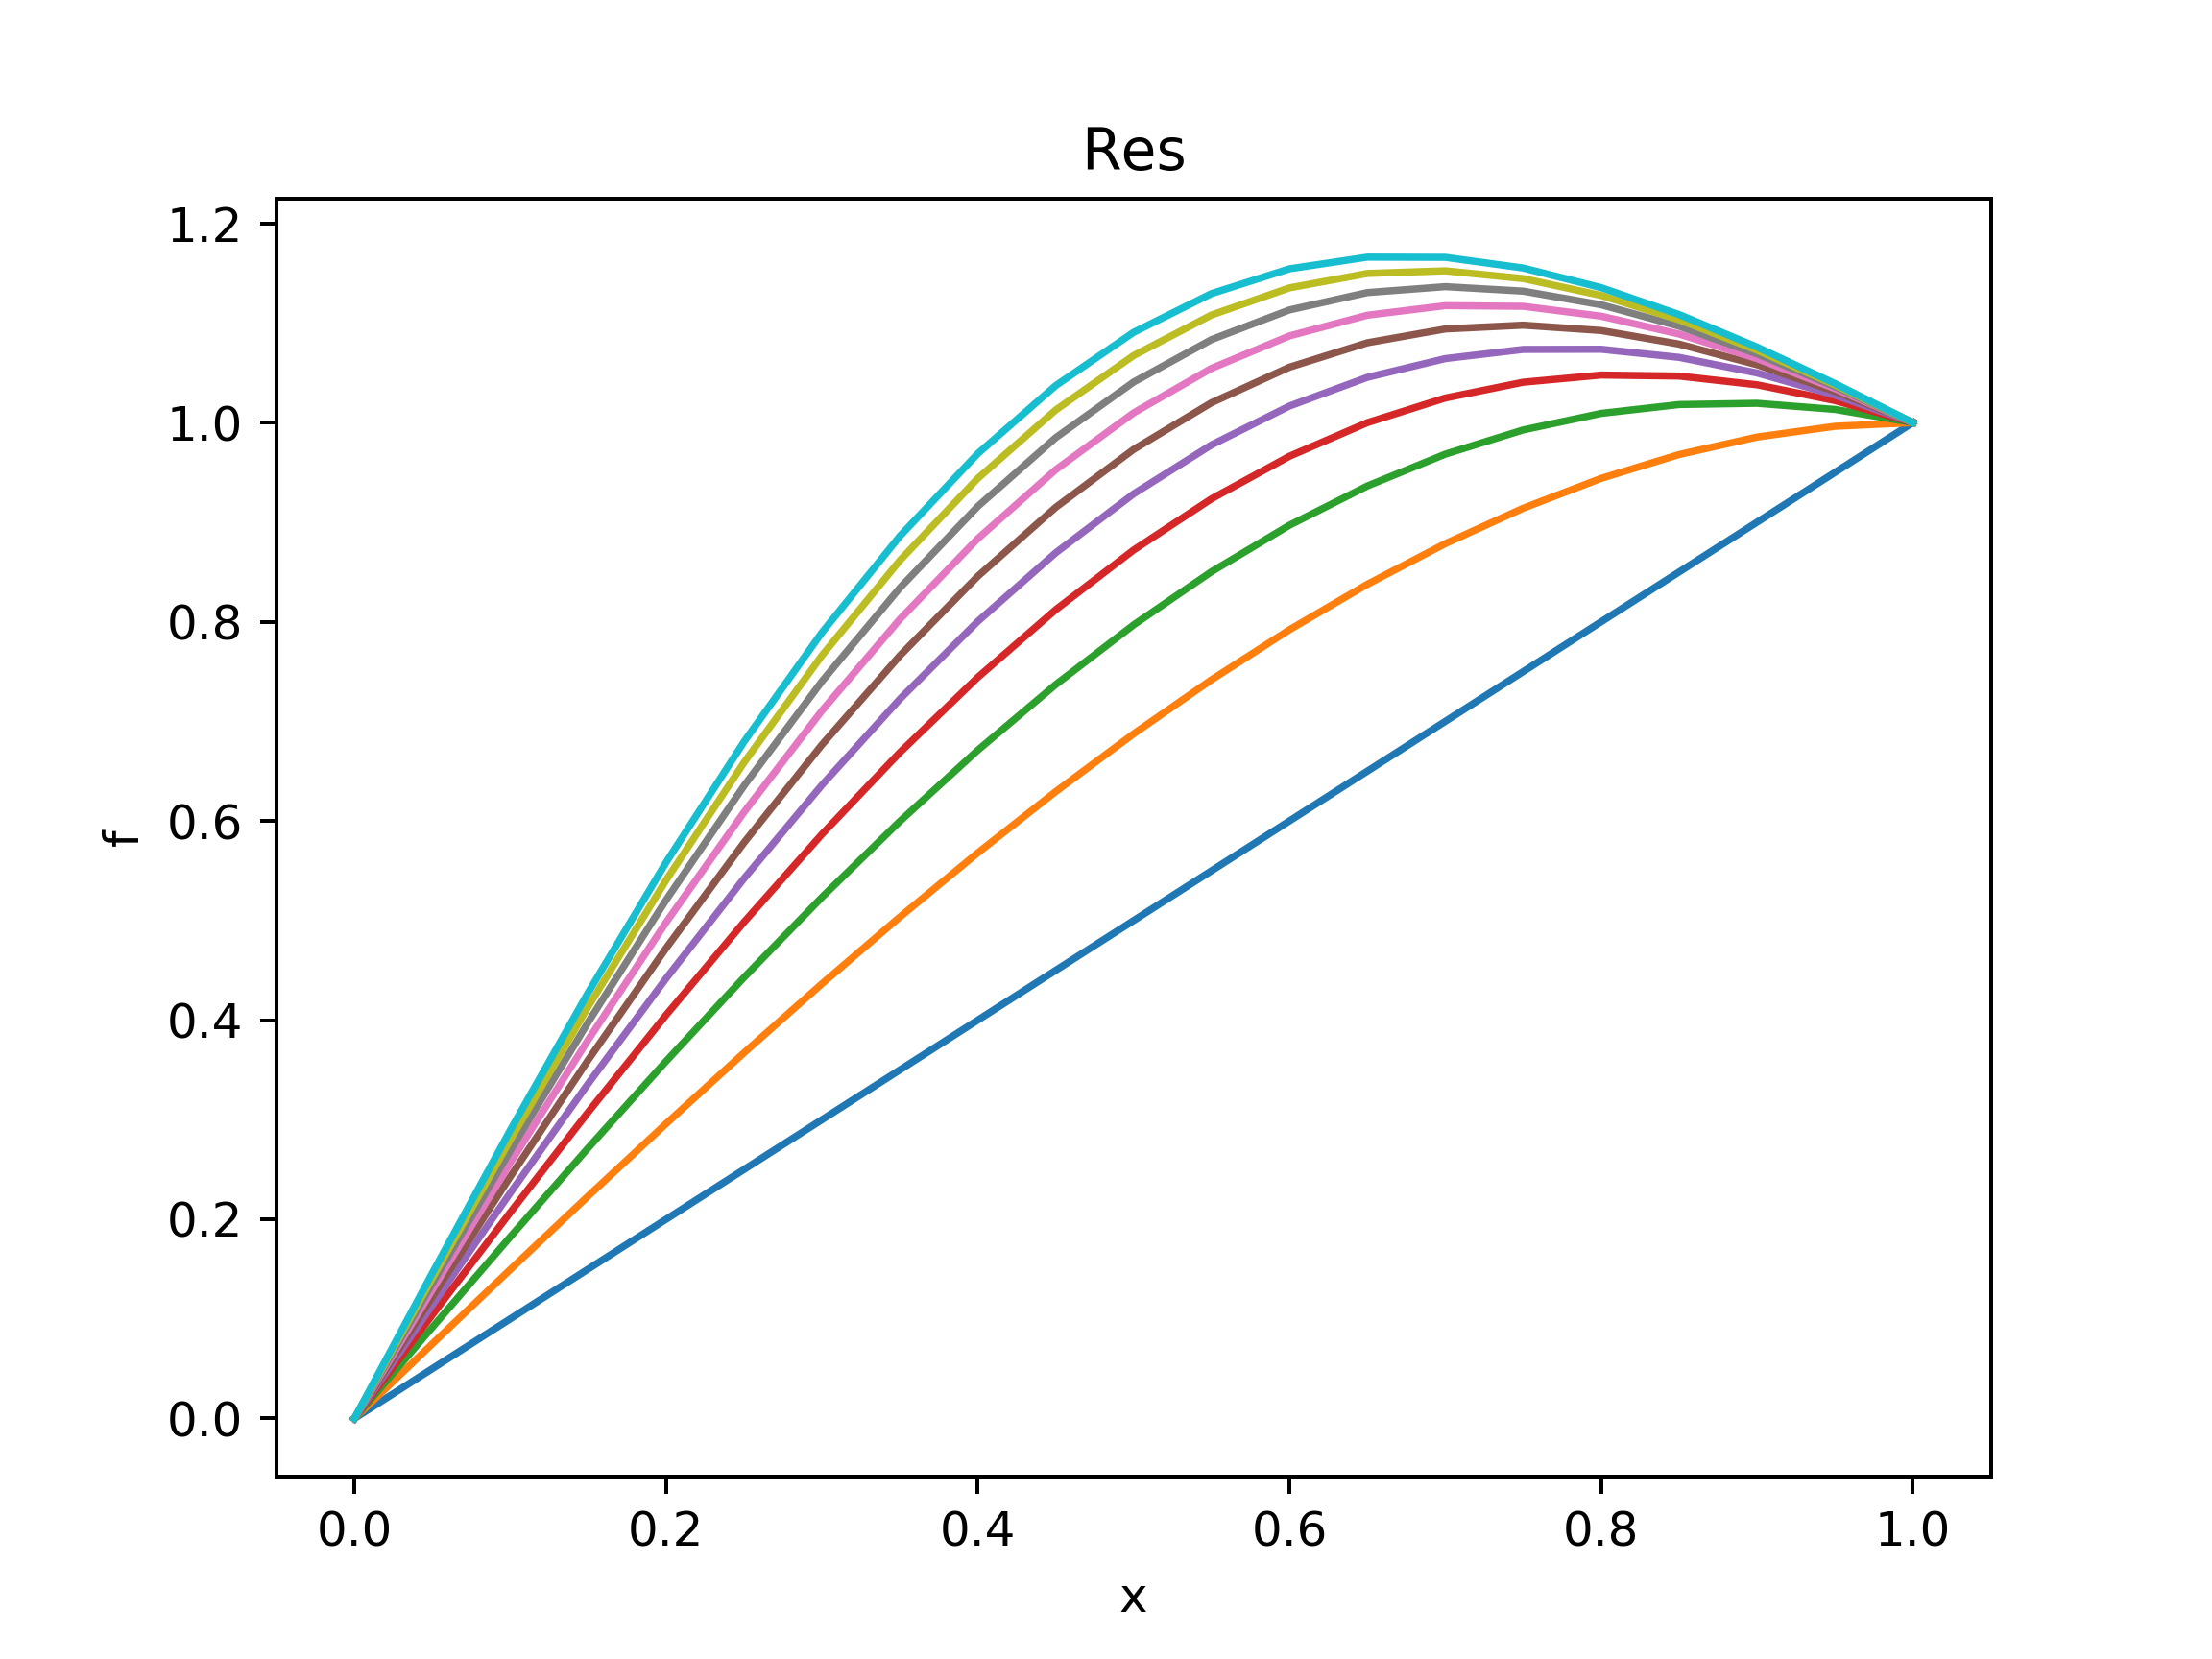
\includegraphics[scale=0.6]{hw3.png}

Code is in attachment. \attachfile{code.py}

$\square$

\end{document}
